\section{Einleitung}

\subsection{Ausgangslage}
Kurze Einführung in die Plattform und Zielsetzung der Applikation.

Beispiel

Wie in Abbildung~\ref{fig:architektur} dargestellt, basiert die Lösung auf einem modularen Aufbau.

\begin{figure}[h]
  \centering
  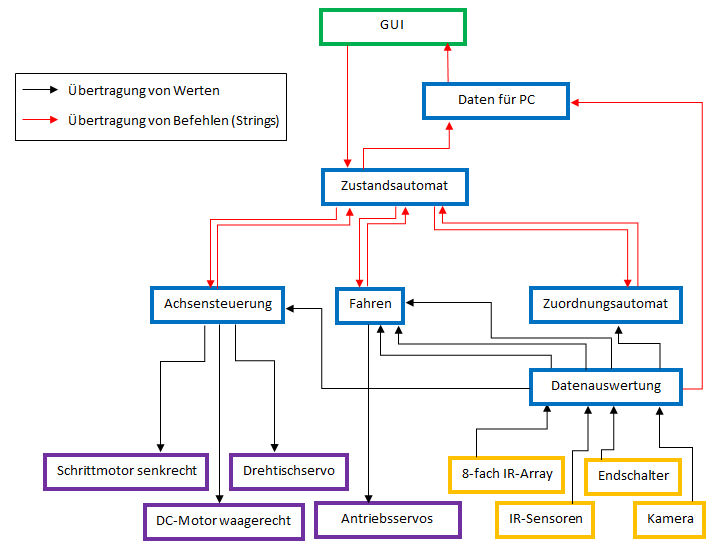
\includegraphics[width=0.8\textwidth]{graphics/software_struktur.png}
  \caption{Systemarchitektur der Lösung}
  \label{fig:architektur}
\end{figure}

\subsection{Monidas}
Beschreibung der Monidas-Plattform

\subsection{Monidas Superuser IP5}
Beschreibung der bestehenden Lösung aus dem IP5

\subsection{Problemstellung}
Beschreibung der Problemstellung

\subsection{Fragestellung}


\subsection{Resultat}
Übersicht über die umgesetzte Lösung

\subsection{Systemübersicht}

\subsection{Systemübersicht}

\textbf{Graphdatenbank}
\begin{itemize}
	\item db.schema …
\end{itemize}

\textbf{Virtuelles Filesystem}
\begin{itemize}
	\item vfs-vscode-extension für VFS
	\item based-vfs
\end{itemize}

\textbf{Language Server Protocol}
\begin{itemize}
	\item lsp-vscode-extension für LSP
	\item based-lsp
\end{itemize}

\subsection{Leserführung}
Was wird wo behandelt?